\begin{landscape}
\section{Alkane (Paraffine)}
\label{sec:Alkane}
\renewcommand{\longtableheader}{\multicolumn{1}{c}{\textbf{Strukturformel}}
&
& \multicolumn{1}{c}{\textbf{vereinfachte Strukturformel}}
& \multicolumn{1}{c}{\textbf{Summenformel}}
& \multicolumn{1}{c}{\textbf{Name}}
\\}
\setatomsep{2em}
\begin{longtable}{cccll}
	\longtableheader
	\endfirsthead
	\longtableheader
	\endhead
	\caption{Ausgewählte Kohlenwasserstoffe}
	\endlastfoot
	\multicolumn{5}{r}{\longtableendfoot} \\
	\endfoot

	\chemfig{H-!{CH2}-H} & & \textdiscount & \tableprintACSandACL{CH4}\vspace{0.3cm} \\
	\chemfig{H-!{CH2}-!{CH2}-H} & & \ce{CH3-CH3} & \tableprintACSandACL{C2H6}\vspace{0.3cm} \\
	\chemfig{H-!{CH2}-!{CH2}-!{CH2}-H} & & \ce{CH3-CH2-CH3} & \tableprintACSandACL{C3H8}\vspace{0.3cm} \\
	\chemfig{H-!{CH2}-!{CH2}-!{CH2}-!{CH2}-H} & & \ce{CH3-CH2-CH2-CH3} & \tableprintACSandACL{C4H10}\vspace{0.3cm} \\
	\chemfig{H-!{CH2}-!{CH2}-!{CH2}-!{CH2}-!{CH2}-H} & & \ce{CH3-CH2-CH2-CH2-CH3}
	&	\tableprintACSandACL{C5H12}\vspace{0.3cm} \\
	\chemfig{H-!{CH2}-!{CH2}-!{CH2}-!{CH2}-!{CH2}-!{CH2}-H} & & \ce{CH3-CH2-CH2-CH2-CH2-CH3}
	&	\tableprintACSandACL{C6H14}\vspace{0.3cm} \\
\end{longtable}
\end{landscape}


\subsection{Definition}
\label{sec:Alkane:Definition}
Alkane sind kettenförmige (azyklische oder aliphatische) Kohlenwasserstoffe (KW) in denen
\ac{6}-Atome nur durch Einfachbindung verbunden sind.

\begin{description}
	\item[Vorsilbe:] Anzahl der \ac{6}-Atome
	\item[Endung:] Einfachbindung zwischen den \ac{6}-Atomen
\end{description}

\subsection{Eigenschaften}
\begin{itemize}
	\item Man nennt sie gesättigte Kohlenwasserstoffe weil die höchst mögliche Anzahl an
		\ac{1}-Atomen eine Verbindung mit dem \ac{6}-Atom eingegangen haben.
	\item Sie wurden früher auch Paraffine (reaktionsträge) genannt.
	\item In Kohlenwasserstoff herrscht eine annähernd reine Atombindung.
%		(Elektronegativitätswerte)
	\item Normalerweise sind, bei Raumtemperatur, alle Stoffe mit reiner Atombindung
		gasförmig. Kohlenstoffverbindungen können auch flüssig oder sogar fest sein.
	\item Je länger die Kette desto träger der Stoff.
\end{itemize}

\begin{center}
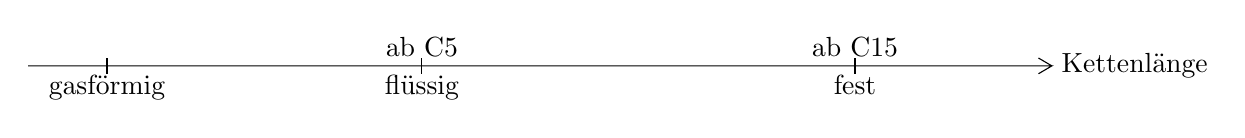
\begin{tikzpicture}
	\draw (0,0.3) -- node[sloped,below] {gasförmig} (2,0.3) -- (2,0.3)
		-- node[sloped,below] {flüssig} node[sloped,above] {ab \ce{C5}} (8,0.3)
		-- node[sloped,below] {fest} node[sloped,above] {ab \ce{C15}} (13,0.3)
		-- (12.83,0.2) -- (13,0.3) -- (12.83,0.4);	%% arrow
	\draw (13,0.3) node[right] {Kettenlänge};
	\draw (1,0.4) -- (1,0.2);
	\draw (5,0.4) -- (5,0.2);
	\draw (10.5,0.4) -- (10.5,0.2);
\end{tikzpicture}
\end{center}

\begin{figurewrapper}
	\href{http://en.wikipedia.org/wiki/File:Methane-3D-balls.png}
	{\includegraphics[width=0.4\hsize]{files/images/Methane-3D-balls}}
	\captionof{figure}{Modell eines \acl{CH4}moleküls}
\end{figurewrapper}
%% Quelle: \url{http://en.wikipedia.org/wiki/File:Methane-3D-balls.png}

\subsection{Alkane bilden eine homologe Reihe}
\label{sec:homologe_Reihe}
Eine Reihe organischer Verbindungen deren Vertreter die gleichen Strukturmerkmale aber
unterschiedliche Kettenlängen haben, deren Vorgänger sich vom Nachfolger durch eine
\ce{CH2}-Gruppe unterscheidet, nennt man homologe Reihe.

Wegen der gleichen Strukturmerkmale sind die chemischen Reaktionen ähnlich.
Wegen unterschiedlicher Kettenlängen sind die physikalischen Eigenschaften verschieden.

\renewcommand{\longtableheader}{\multicolumn{1}{l}{\textbf{Formel}}
& \multicolumn{1}{l}{\textbf{Name}}
& \multicolumn{1}{l}{\textbf{Schmelz-}}
& \multicolumn{1}{l}{\textbf{Siede-}}
%& \multicolumn{1}{l}{\textbf{Flamm-}}
& \multicolumn{1}{l}{\textbf{Aggregat-}}
%& \multicolumn{1}{l}{\textbf{Dichte}}
& \multicolumn{1}{l}{\textbf{Viskosität}} \\
&
& \multicolumn{1}{l}{\textbf{temp. (\si{\degreeCelsius})}}
& \multicolumn{1}{l}{\textbf{temp. (\si{\degreeCelsius})}}
%& \multicolumn{1}{l}{\textbf{temp. (\si{\degreeCelsius})}}
& \multicolumn{1}{l}{\textbf{zustand}}
%& \multicolumn{1}{l}{\textbf{(\si{\gram\per\square\centi\metre})}}
& \\
}
\begin{longtable}{llrrlc}
	\longtableheader
	\endfirsthead
	\longtableheader
	\endhead
	\caption{Eigenschaften Ausgewählte Kohlenwasserstoffe}
	\endlastfoot
	\multicolumn{6}{r}{\longtableendfoot} \\
	\endfoot

	\tableprintACSandACL{CH4}		& $-184$	& $-164$	& Gas		& \\
	\tableprintACSandACL{C2H6}		& $-172$	& $-89$		& Gas		& \\
	\tableprintACSandACL{C3H8}		& $-190$	& $-42$		& Gas		& \\
	\tableprintACSandACL{C4H10}		& $-135$	& $-0,5$	& Gas		& \\
	\tableprintACSandACL{C5H12}		& $-129$	& 36	& flüssig	& \\
	\tableprintACSandACL{C6H14}		& $-94$		& 69	& flüssig	& \\
	\tableprintACSandACL{C7H16}		& $-90$		& 98	& flüssig	& \\
	\tableprintACSandACL{C8H18}		& $-59$		& 126	& flüssig	& \\
	\tableprintACSandACL{C9H20}		& $-54$		& 151	& flüssig	& \\
	\tableprintACSandACL{C10H22}	& $-30$		& 174	& flüssig	& \\
	\tableprintACSandACL{C11H24}	& $-26$		& 196	& flüssig	& \\
	\tableprintACSandACL{C12H26}	& $-10$		& 216	& flüssig	& \\
	\tableprintACSandACL{C13H28}	& $-6$		& 230	& flüssig	& \\
	\tableprintACSandACL{C14H30}	& 5,5	& 251	& flüssig	& \\
	\tableprintACSandACL{C15H32}	& 10	& 268	& flüssig	& \\
	\tableprintACSandACL{C16H34}	& 18	& 280	& fest		& \\
	\tableprintACSandACL{C17H36}	& 22	& 303	& fest
		&  \multirow{-18}{*}{\rotatebox{-90}{$\autorightarrow{nimmt zu}{}$}} \\
\end{longtable}


\begin{itemize}
	\item organische Stoffe
	\item gleiche chemische Reaktion
	\item unterschiedliche physikalische Eigenschaften
\end{itemize}

\cVersuch{2}{Verbrennung von Alkanen}
\begin{description}
	\item[Aufbau:] 5 Abdampfschalen, Bunsenbrenner, Holzstäbchen, Dreifuß, \\
		\ac{C5H12}, \ac{C6H14}, \ac{C7H16}, \ac{C8H18}, \ac{C17H36}.
	\item[Durchführung:] Wir versuchten die Alkane nacheinander anzuzünden.
	\item[Beobachtung:]~
	\begin{list}{}{}
		\item[\ac{C5H12}:] Flüssig, durchsichtig, riecht nach Benzin, \\
			ist sehr leicht entzündbar, orange Flamme.
		\item[\ac{C6H14}:] wie das \ac{C5H12}.
		\item[\ac{C7H16}:] etwas dickflüssig, öliger, durchsichtig, riecht nach Benzin, \\
			etwas langsamer entzündbar, brennt orange.
		\item[\ac{C8H18}:] öliger, riecht weniger nach Benzin, durchsichtig, \\
			schwerer entzündbar, brennt orange
		\item[\ac{C17H36}:] sehr ölig, dickflüssig, durchsichtig, \\
			mit Holzspan nicht entzündbar, auch nicht mit einer
			Bunsenbrennerflamme \\
			in unserem Experiment ließ es sich nicht entzünden. Eigentlich geht etwas von
			dem \ac{C17H36} in den gasförmigen Zustand über. Folglich ließe sich das
			\ac{C17H36}-Gas mit einem Holzspan entzünden.
	\end{list}
\end{description}

\begin{description}
	\item[Flammenvergleich:]~
	\begin{itemize}
		\item Die Flamme des \ac{CH4} (Bunsenbrenner) ist blau.
		\item Die anderen Flammen sind gelb-orange.
		\item Bei zunehmendem Kohlenstoffanteil wird die Flamme immer orangefarbener.
		\ifDraft{\item Je länger die Atomkette desto mehr Kohlenstoffanteil.
			\fxwarning{true ???}}{}
		\item In den Abdampfschalen bleibt unverbrannter Ruß (\ac{6}) zurück.
	\end{itemize}
	\item[Geruchsprobe:] Gasförmige und Feste Alkane sind geruchsfrei, Flüssige riechen
		nach Benzin.
	\item[Gleichungen:]
	\begin{align}
		\ce{CH4 + 2O2}			& \ce{-> CO2 + 2H2O} \\
		\ce{C2H6 + O2}			& \ce{-> CO2 + H2O} \\
		\ce{2C2H6 + 7O2}		& \ce{-> 4CO2 + 6H2O} \\
		\ce{C3H8 + 5O2}			& \ce{-> 3CO2 + 4H2O}
	\end{align}
	\begin{align}
		\ce{C6H14 + 19/2O2}		& \ce{-> 6CO2 + 7H2O} \\
		\ce{2C6H14 + 19O2}		& \ce{-> 12CO2 + 14H2O}
	\end{align}
\end{description}

\vspace{-0.5cm}
Bei gerader \ac{6}-Anzahl mit 2 erweitern, weil sonst Brüche in der Gleichung vorkommen.

\cVersuch{2}{Löslichkeit in \acl{H2O}}
\begin{description}
	\item[Überlegung:] Alkane sind eine Erdölfraktion. Kurzkettige Alkane haben einen
		ähnlichen Aggregatzustand und Konsistenz wie \ac{H2O}.
	\item[Aufbau:] \ac{C5H12}, \ac{H2O}, Reagenzglas.
	\item[Beobachtung:]~
	\begin{itemize}
		\item Trennschicht (schlecht in \ac{H2O} löslich: Hydrophob).
		\item bei Schütteln, kurzzeitige Emulsion.
	\end{itemize}
\end{description}

\begin{figurewrapper}
	\includegraphics[width=0.15\hsize]{files/pst-labo/Pentan-pics}
	\captionof{figure}{\acl{C5H12} in \acl{H2O}}
\end{figurewrapper}

Alkane reagieren weder auf die stärkste Lauge (Alkalilauge) noch auf die
stärkste Säure \ac{H2SO4}.

\cVersuch{2}{Alkan und Halogen}
\begin{description}
	\item[Aufbau:] \ac{C6H14}, \ac{Br2}, Becherglas,
		angefeuchtetes Indikatorpapier (Lackmuspapier) ist oben am Becherglas befestigt,
		Pipette, Dreifuß, Bunsenbrenner.
	\item[Vorüberlegung:] Bei einfachem zusammengießen der beiden Stoffe wird nichts geschehen,
		da \ac{Br2} nur durch Licht oder Wärme reagiert. Da \ac{Br2} ein Nichtmetall ist,
		sollte sich, falls eine Reaktion zu Stande kommt, das Lackmuspapier rot Färben.
		\newpage
	\item[Durchführung:]~ \vspace{-2em}
	\begin{figure}[H]\centering
		\includegraphics[width=0.12\hsize]{files/pst-labo/Brom+Hexan-pics}
		\captionof{figure}{\acl{Br2} reagiert mit \acl{C6H14}}
	\end{figure}\vspace*{-1em}
	\item[Beobachtung:]~
	\begin{itemize}
		\item zuerst keine Reaktion.
		\item während dem erhitzen mit dem Bunsenbrenner entsteht Gas, dass das
			Indikatorpapier rot färbt.
		\item Das Brom-Alkangemisch entfärbt sich.
	\end{itemize}
	\item[Gleichung:] \chemfig{H-!{CH2}-!{CH2}-!{CH2}-!{CH2}-!{CH2}-!{CH2}-H}
		\chemsign{+} \ce{\lewis{246,Br}-\lewis{026,Br}} \\[0.8ex]
		\ce{->}\hspace{0.175cm} \chemfig{H-!{CH2}-!{CH2}-!{CH2}-!{CH2}-!{CH2}-!{CH2}-\lewis{026,Br}}
		\chemsign{+} \ce{H-\lewis{026,Br}} \\[0.8ex]
		Es entsteht 1-Monobromhexan und \ac{HBr}.
	\item[Erklärung:] Durch die Spaltung sind die Außenelektronen frei geworden.
		Da die Spaltung genau in der Mitte erfolgte, handelt es sich um eine homolytische Spaltung.
		%% Es entstehen...
		Ein \ac{1}-Atom wird durch ein \ac{35}-Atom ausgetauscht.
\end{description}

\subsection{Substitution}
Die Substitution ist eine chemische Reaktion bei der Atome oder Atomgruppen durch andere ausgetauscht
werden.

Stoffe die sich ablagern sind Substituenten.

Es entstehen immer wieder neue Abspaltungen bis alle \ac{1}-Atome von den Kohlenstoffatomen abgespalten
sind und sich stattdessen Halogene ablagern.

\donkeybridge{zur Substitution: \enquote{aus zwei mach zwei}}

\cVersuch{2}{Beilsteinprobe -- Nachweis von Halogenalkanen}
Entwickelt Anfang des 19 Jahrhundert vom Chemiker Friedrich Konrad Beilstein.

\begin{description}
	\item[Aufbau:] Abdampfschale, Bunsenbrenner, \ac{29}-Streifen, Tiegelzange, Monobromhexan.
	\item[Durchführung:]~
	\begin{enumerate}
		\item Ausglühen eines \ac{29}-Streifens über dem Bunsenbrenner (um zu verhindern, dass die grüne
			Kupferflamme den Nachweis stört).
		\item \ac{29} in das Halogenalkan (CFKW) halten.
		\item Dann in die rauschende Bunsenbrennerflamme halten.
	\end{enumerate}
	\item[Beobachtung:] Die Flamme glüht erst gelb und dann blau-grün (Halogenalkannachweiß)
	\item[Erklärung:] Die gelbe Flamme erscheint durch übermäßiges Hexan. Die blau-grüne Flamme wird
		durch die Kupferhalogene hervorgerufen.
\end{description}

\subsection{Erstsubstitution}
Am Beispiel von \ac{C2H6} und \ac{Cl2}.

\chemfig{H-!{CH2}-!{CH2}-H} \chemsign{+} \ce{\Lewis{246,Cl}-\Lewis{026,Cl}}
\chemsign{\ce{->}} \chemfig{H-!{CH2}-C(-[::90]\lewis{024,Cl})(-[::-90]H)-H} \chemsign{+}
\ce{H-\lewis{026,Cl}}

%Zwischen den \ac{6} annähernd reine Atombindung

\subsection{Zweisubstitution}
Man muss von der Erstsubstitution ausgehen.

\chemfig{H-!{CH2}-C(-[::90]\lewis{024,Cl})(-[::-90]H)-H} \chemsign{+} \ce{\Lewis{246,Cl}-\Lewis{026,Cl}}
\chemsign{\ce{->}} \chemfig{H-C(-[::90]H)(-[::-90]\lewis{046,Cl})-C(-[::90]\lewis{024,Cl})(-[::-90]H)-H}
\chemsign{+} \ce{H-\lewis{026,Cl}}

\vspace{0.3ex}
Die \ac{17}-Atome sind aufgrund ihrer gleichen Außenelektronen, die sich abstoßen, so weit wie möglich
entfernt. Dies ist die stabilste Anordnung.

\begin{minipage}{0.3\hsize}
	\definesubmol{CCl2lewis}{C(-[::90]\lewis{024,Cl})(-[::-90]\lewis{046,Cl})}
	\chemfig{\lewis{246,Cl}-!{CCl2lewis}-!{CCl2lewis}-!{CCl2lewis}-\lewis{026,Cl}}
\end{minipage}\hfill
\begin{minipage}{0.6\hsize}
	Dieses Halogenalkan ist unter normalen Umständen nicht lange beständig.
%	da sich die gleich geladenen
\end{minipage}

\vspace{0.3ex}
Man nennt diese Alkane voll substituierte Alkane.
Voll substituierte Alkane brennen nicht (gasförmig).
Sie sind daher in Feuerlöschern benutzt worden.
Die meisten sind allerdings Krebs erregend.
\ifDraft{Sie sind Stabiler als Alkane gleicher Kettenlänge.
\fxwarning{true ???}}{}

%\subsection{Vereinfachte Strukturformel}
\fxnote{Im Epochenheft ist hier ein Beispiel zu der vereinfachten Strukturformel}
%% 7610

\subsection{Benennung von Halogenalkanen}
\begin{description}
	\item[Beispiel:] \chemfig{H-C(-[::90]\lewis{024,Cl})(-[::-90]\lewis{046,Br})
			-C(-[::90]\lewis{024,Br})(-[::-90]\lewis{046,Cl})
			-C(-[::90]\lewis{024,F})(-[::-90]H)
			-C(-[::90]H)(-[::-90]\lewis{046,F})-H}
		\hspace{3em} 1,2-Dibrom-1,2-Dichlor-3,4-Diflourbutan
\end{description}

\begin{enumerate}
	\item Längste \ac{6}-Kette benennen und (nach Stellung der Substituenten)
		vom kürzesten Kettenende an durchnummerieren; Substituenten werden im
		Namen in alphabetischer Reihenfolge angegeben.
	\item Stellung der Substituenten als Zahl angeben.
		(Stellung der \ac{6}-Atome durch Zahlen muss nicht angegeben werden,
		wenn nur ein \ac{6} vorhanden ist.)
	\item Anzahl der gleichen Halogenalkane mit griechischem Zahlwort angeben.
	\item Endung: -an; % da zwischen
		nur Einfachbindungen.
\end{enumerate}

\subsubsection{Griechische Zahlwörter}
\begin{multicols}{4}
\begin{enumerate}
	\item mon(o)
	\item di
	\item tri
	\item tetra
	\item pent(a)
	\item hex(a)
	\item hept
	\item okt
	\item non(a)
	\item dek(a)
	\item undek
	\item dodek
	\item tridek
	\item tetradek
	\item pentadek
	\item hexadek
\end{enumerate}
\end{multicols}

\subsection{Isomerie der Alkane}
Unterschiedliche Strukturen verursachen unterschiedliche Eigenschaften
(zum Beispiel unterschiedliche Siedetemperaturen)

Isomere sind Stoffe mit gleicher Summenformel, aber unterschiedlicher Strukturformel.

Das Auftreten dieser Erscheinungsform nennt man Isomerie.

\begin{itemize}
	\item Ab \ac{C4H10} gibt es Isomere.
	\item Bei einem Alkan mit 25 \ac{6}-Atomen gibt es 36 Millionen Isomerie-Möglichkeiten.
\end{itemize}

\subsubsection{Beispiel}
\begin{multicols}{2}
\chemname{\chemfig{H-!{CH2}-!{CH2}-!{CH2}-!{CH2}-H}}{N-Butan (Normalbutan)}

\chemname{\chemfig{H-!{CH2}-C(-[::+90]H)(-[::-90,2]C(-H)(-[::-90]H)-[::0]H)-!{CH2}-H}}{Methylpropan}
\end{multicols}

\subsubsection{Namensgebung bei Isomeren}
\begin{multicols}{2}
\chemfig{CH_3-C(-[::90]CH_3)(-[::-90]CH_3)-CH([::-90]-CH_2-CH_3)-CH_2-CH_2-CH_2-CH_3}

3-Ethyl-2,2-Dimethylheptan
\end{multicols}

\begin{enumerate}
	\item Hauptkette ermitteln und benennen (längste Kette).
	\item Seitenkette benennen und alphabetisch ordnen
		(Endung: -yl statt -an; Alkylrest: Radikale, die sich aus den Alkanen ableiten,
		aus denen sie durch Entzug eines \ac{1}-Atoms entstehen: $\mathrm{C_nH_{2n+1}}$).
	\item Anzahl gleicher Seitenketten mit Zahlwort kennzeichnen (-di, -tri, -tetra).
	\item Verknüpfungstelle zwischen Haupt- und Seitenkette angeben (vom kürzesten
		Kettenende an zählen).
\end{enumerate}

\renewcommand{\longtableheader}{\multicolumn{1}{c}{\textbf{Name}}
& \multicolumn{1}{c}{\textbf{vereinfachte}}
& \multicolumn{1}{l}{\textbf{Siede-}}	\\

& \multicolumn{1}{c}{\textbf{Strukturformel}}
& \multicolumn{1}{l}{\textbf{temp. (\si{\degreeCelsius})}}
\\[0.5ex]}
\begin{longtable}{lcr}
	\longtableheader
	\endfirsthead
	\longtableheader
	\endhead
	\caption{Übungen zum aufstellen der vereinfachten Strukturformel}
	\endlastfoot
	\multicolumn{3}{r}{\longtableendfoot} \\
	\endfoot

	n-Hexan				& \ce{CH3-CH2-CH2-CH2-CH2-CH3}							& 69 \\[0.5ex]
	2-Methylpentan		& \chemfig{CH_3-CH(-[::-90]CH_3)-CH_2-CH_2-CH_3}		& 60 \\
	3-Methylpentan		& \chemfig{CH_3-CH_2-CH(-[::90]CH_3)-CH_2-CH_3}			& 63 \\[0.8ex]
	2,2-Dimethylbutan	& \chemfig{CH_3-C(-[::90]CH_3)(-[::-90]CH_3)-CH_2-CH_3}	& 50 \\[6.75ex]
	2,3-Dimethylbutan	& \chemfig{CH_3-CH(-[::90]CH_3)-CH(-[::-90]CH_3)-CH_3}	& 58 \\
\end{longtable}

Ist die Zahl der \ac{6}-Atome gleich, so ist die Siedetemperatur um so niedriger,
je stärker verzweigt das Alkan ist.

Warum sinkt die Siedetemperatur bei zunehmender Verzweigung?
\begin{itemize}
	\item maximale Abstoßung.
	\item Mit abnehmender Oberfläche sieden die Stoffe besser.
\end{itemize}
